%\title{LaTeX Portrait Poster Template}
%%%%%%%%%%%%%%%%%%%%%%%%%%%%%%%%%%%%%%%%%
% a0poster Portrait Poster
% LaTeX Template
% Version 1.0 (22/06/13)
%
% The a0poster class was created by:
% Gerlinde Kettl and Matthias Weiser (tex@kettl.de)
% 
% Adapter by Jens Buysse for Hogeschool Gent
% This template has been downloaded from:
% http://www.LaTeXTemplates.com
%
% License:
% CC BY-NC-SA 3.0 (http://creativecommons.org/licenses/by-nc-sa/3.0/)
%
%%%%%%%%%%%%%%%%%%%%%%%%%%%%%%%%%%%%%%%%%

%----------------------------------------------------------------------------------------
%	PACKAGES AND OTHER DOCUMENT CONFIGURATIONS
%----------------------------------------------------------------------------------------

\documentclass[a0,portrait]{a0poster}

\usepackage{multicol} % This is so we can have multiple columns of text side-by-side
\columnsep=100pt % This is the amount of white space between the columns in the poster
\columnseprule=3pt % This is the thickness of the black line between the columns in the poster

\usepackage[svgnames]{xcolor} % Specify colors by their 'svgnames', for a full list of all colors available see here: http://www.latextemplates.com/svgnames-colors

\usepackage{times} % Use the times font
%\usepackage{palatino} % Uncomment to use the Palatino font

\usepackage{graphicx} % Required for including images
\graphicspath{{figures/}} % Location of the graphics files
\usepackage{booktabs} % Top and bottom rules for table
\usepackage[font=small,labelfont=bf]{caption} % Required for specifying captions to tables and figures
\usepackage{amsfonts, amsmath, amsthm, amssymb} % For math fonts, symbols and environments
\usepackage{wrapfig} % Allows wrapping text around tables and figures
\usepackage[export]{adjustbox}

\begin{document}

%----------------------------------------------------------------------------------------
%	POSTER HEADER 
%----------------------------------------------------------------------------------------

% The header is divided into two boxes:
% The first is 75% wide and houses the title, subtitle, names, university/organization and contact information
% The second is 25% wide and houses a logo for your university/organization or a photo of you
% The widths of these boxes can be easily edited to accommodate your content as you see fit

\begin{minipage}[t]{0.75\linewidth}
\VeryHuge \color{HoGentAccent1} \textbf{Een vergelijkende studie tussen gRPC met Protocol Buffers en REST met JSON in opdracht van Fashion Society.} \color{Black}\\ % Title
\Huge\textit{}\\[2.4cm] % Subtitle
\huge \textbf{Pepermans Sven, Kristof Van Moorter, Antonia Pierreux}\\[0.5cm] % Author(s)
\huge Hogeschool Gent, Arbeidstraat 14, 9300 Aalst\\[0.4cm] % University/organization
\Large \texttt{sven.pepermans@student.hogent.be} \\
\end{minipage}
%
\begin{minipage}[t]{0.25\linewidth}
\includegraphics[width=13cm,right]{figures/HOGENT_Logo_Pos_rgb.png} 

\end{minipage}

\vspace{1cm} % A bit of extra whitespace between the header and poster content

%----------------------------------------------------------------------------------------

\begin{multicols}{2} % This is how many columns your poster will be broken into, a portrait poster is generally split into 2 columns

%----------------------------------------------------------------------------------------
%	ABSTRACT
%----------------------------------------------------------------------------------------

\color{HoGentAccent1} % Navy color for the abstract

\begin{abstract}
In dit onderzoek worden REST met JSON en gRPC met Protocol Buffers onderzocht en met elkaar vergeleken. Voor het uitvoeren van dit onderzoek wordt gebruik gemaakt van de testserver van de Fashion Society waar de huidige structuur reeds op geïmplementeerd is. De twee structuren worden vergeleken op basis van performantie in twee groeperingen, de kleine payload bestaande uit vierduizend requests en de grote payload bestaande uit tienduizend requests.
\end{abstract}
%----------------------------------------------------------------------------------------
%	INTRODUCTION
%----------------------------------------------------------------------------------------

\color{HoGentAccent1} 
\section*{Introductie}
\color{black}
\color{black}
De Fashion Society, het overkoepelende bedrijf van wel gekende kledingketens zoals ZEB en The Fashion Store is een bedrijf dat in constante groei zit, zijnde het door overnames of door het zelf openen van nieuwe winkels. Hoe meer winkels, hoe meer data, hoe meer intern dataverkeer en tot slot hoe meer nood aan efficiëntie.

Momenteel maakt de Fashion Society intern gebruik van eigen microservices met behulp van REST en Json. Json is wereldwijd één van de meest gebruikte dataformaten echter wil dit niet zeggen dat dit het snelste is, laat staan het efficiëntste in samenwerking met REST. In dit onderzoek wordt er dan ook onderzocht of gRPC met Protocolbuffers al dan niet performanter is dan REST met Json.

\begin{center}\vspace{1cm}
	
\includegraphics[width=1.0\linewidth]{Fashion_society}
	\captionof{figure}{\color{HoGentAccent5}Fashion Society}
\end{center}\vspace{1cm}

Dit onderzoek is in opdracht van Fashion Society en de Proof-Of-Concept is opgesteld met bijstand Kristof Van Moorter, Developer voor Fashion Society.
%----------------------------------------------------------------------------------------
%	GEOLOGY
%----------------------------------------------------------------------------------------

\color{Black} % DarkSlateGray color for the rest of the content
\color{HoGentAccent1} 
\section*{Onderzoek}
\color{black}
Voor deze bachelorproef is er in twee delen gewerkt, namelijk een literatuurstudie waarin de nodige context wordt uitgelegd om deze bachelorproef te kunnen volgen en een tweede deel bestaande uit een Proof-Of-Concept en de bijhorende resultaten.

In de Proof-Of-Concept zijn drie scenario's getest. Het eerste scenario is het verschil in performantie op basis van één enkele call. Deze test is tienduizend keer uitgevoerd om eventuele netwerkvertragingen en dergelijke anomalieën te vermijden.
Het tweede scenario is het verschil in performantie op basis van een kleine payload, zijnde vierduizend parallelle calls. Dit scenario is net zoals het derde scenario, het verschil in performantie op basis van een grote payload, zijnde tienduizend parallelle calls, 4 keer uitgevoerd. 

\begin{center}\vspace{1cm}
	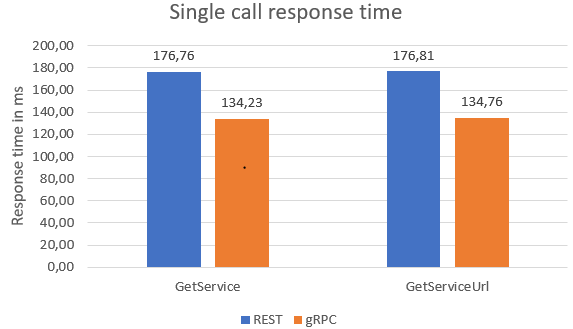
\includegraphics[width=1.0\linewidth]{singleCall}
	\captionof{figure}{\color{HoGentAccent5}De resultaten van de Proof-Of-Concept voor één enkele call.}
\end{center}\vspace{1cm}


%------------------------------------------------



\color{HoGentAccent1} 
\section*{Conclusies}
\color{black}
Na het uitvoeren van de Proof-Of-Concept en het analyseren van de resultaten is de conclusie tot stand gekomen dat gRPC met ProtocolBuffers sneller en performanter is dan REST met Json voor de implementatie van Fashion Society. Op de onderzoeksvraag “Is gRPC met ProtocolBuffers efficiënter dan REST API met JSON op gebied van CPU gebruik voor de implementatie van de Fashion Society?” kan geen antwoord gegeven worden omdat deze gegevens niet exact meetbaar waren gedurende het uitvoeren van de proof-of-concept.
%----------------------------------------------------------------------------------------
%	FORTHCOMING RESEARCH
%----------------------------------------------------------------------------------------
\color{HoGentAccent1} 
\section*{Toekomstig onderzoek}
\color{black}

Dit onderzoek heeft zich enkel gericht op de communicatie tussen de Orchestrator API en Discovery API van de Fashion Society. Toekomstig onderzoek kan gedaan worden naar de performantie in communicatie tussen de interne services en de Discovery API voor de huidige REST implementatie en een gRPC implementatie.

Alsook kan toekomstig onderzoek gedaan worden naar de winst in performantie bij het omschakelen naar een volledige gRPC structuur waarbij REST en JSON nog amper tot niet meer gebruikt worden. Echter zal dit laatste onderzoek in praktijk moeilijk te behalen zijn door de omvang van het huidige aantal REST services binnen de Fashion Society.


%----------------------------------------------------------------------------------------

\end{multicols}
\end{document}